\newcommand{\mess}[3] {
\begin{figure}[H]
	\centering
	\includegraphics[width=0.7\textwidth]{#1}
	\caption{#2}
	\label{#3}
\end{figure} }
\newcommand{\refabb}[1]{(siehe Abb. \ref{#1})}

\chapter{Versuchsdurchführung}
\section{Testschaltungen}
\subsection{Verstärkungsfaktor einer nicht-invertierenden Schaltung}
Zur Vorbereitung auf die Benutzung der Operationsverstärker in der Ekg
Schaltung, messen wir Ein- und Ausgangsspannung einer Impedanzwandlerschaltung
und einer nicht-invertierenden Verstärkerschaltung.\\
\begin{figure}[htb]
    \centering
    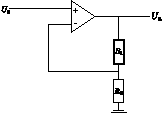
\includegraphics[width=0.6\textwidth]{Abb/nicht-inv.pdf}
    \caption{Schaltung einer nicht-invertierenden Verstärkerschaltung. Die
Verstärkung wird durch das Verhältnis der beiden Widerstände zueinander
bestimmt.}
    \label{ninv}
\end{figure}

Zur Messung benutzen wir ein Signalinterface, um ein Messsignal von
$\SI{0}{\volt}$ bis $\SI{5}{\volt}$ zu generieren und den Output wieder
abzutasten. \\
\mess{Mess/Op/faktor1.pdf}{Messung einer Impedanzwandlerschaltung. Die
						   Verstärkung ist 1. Diese Schaltung wird benutzt um den hohen Widerstand des
						   Körpers vor der Verstärkung des Ekg Signals zu kompensieren.}{imp}

Zur Messung hoher Verstärkungen benutzen wir einen Spannungsteiler vor dem
Eingang des Verstärkers. In Abbildung \ref{spann} ist das Signal nur durch den
Spannungsteiler zu sehen.\\
\mess{Mess/Op/spannungsteiler.pdf}{Messung des benutzten Spannungsteiler am
Eingang}{spann}

Zur Messung der nicht-invertierenden Verstärkerschaltung benutzten wir vier
unterschiedliche Widerstandsverhältnisse. 
	\begin{table}[H]
		\centering
		\begin{tabular}{|c c c|}
			\hline
			$R_1$ &$R_2$ &Verstärkung \\ \hline
			$\SI{1}{\kilo \ohm}$ &$\SI{10}{\kilo\ohm}$ &$1.1$ \\
			$\SI{33}{\kilo\ohm}$ &$\SI{10}{\kilo\ohm}$ &$4.3$ \\
			$\SI{47}{\kilo\ohm}$ &$\SI{10}{\kilo\ohm}$ &$5.7$ \\
			$\SI{100}{\kilo\ohm}$ &$\SI{10}{\kilo\ohm}$ &$11$ \\
			\hline
		\end{tabular}
	\end{table}

In Abbildung \ref{noninv} ist zu erkennen, dass die Verstärkung im Rahmen der Messtoleranz
gut erreicht wurde.\\
\mess{Mess/Op/noninv.pdf}{Messung der nicht-invertierenden Verstärkerschaltung.
In der Legende sind die Verstärkungen des jeweiligen Aufbaus gelistet. Zur
Messung wurde ein Spannungsteiler am Eingang verwendet, um die maximale Spannung
des AD-Wandlers nicht zu überschreiten.}{noninv}

\subsection{Frequenzfilter}
Die Filter im Praktikumsraum haben nicht funktioniert. Aus diesem Grund wurden
die Testschaltungen zu Frequenzfilter mit einem selbstzusammengeschalteten
Hochpassfilter, bestehend aus einem Kondensator und einem Widerstand,
durchgeführt. \\
\begin{figure}[htb]
	\centering
	\includegraphics[width=0.7\textwidth]{Mess/hochpass.pdf}
	\caption{Messung des Hochpass', Linie bei $\frac{1}{\sqrt{2}} \; U_{ein}$}
	\label{hochuf}
\end{figure}

Um die Ordnung des Hochpass' zu bestimmen, soll zunächst der Spannungsabfall in
der linearen Region des Filters. Zwischen $\SI{8}{\hertz}$ und $\SI{5}{\hertz}$
fällt die Spannung von $\SI{3,44}{\volt}$ auf $\SI{1,24}{\volt}$ ab. In
Dezibel
\[
Q_{(U)} = 10 \cdot \lg \frac{3,44}{1,24} \si{\decibel} = \SI{4,43}{\dB}
\]
Um nun den Abfall pro Dekade zu erhalten, rechnet man
\[
\frac{Q_{(U)} }{\text{Dekade}} = \frac{ \SI{4,43}{\dB} }{ \SI{6}
{\Hz}} \cdot \frac{ 180 \text{Hz} }{\text{Dekade}} = 133 \, \frac{
\si{\dB}}{\text{Dekade}}
\]
Für die Ordnung gilt weiter
\[
\frac{ \SI{20}{\dB} }{\text{Dekade} \cdot \text{Ordnung} }
\]
Somit handelt es sich bei unserem Filter um einen Hochpass der Ordnung 6.
Die Grenzfrequenz beträgt dem Graphen zufolge ca 14 Hz. 

\section{EKG Schaltung}

Durch das Fehlen der Frequenzfilter liegen die Messdaten des EKGs sehr
verrauscht vor. Dennoch kann man in Abbildung \ref{jon1} und \ref{kor1} die
Schläge erkennen. 
\mess{Mess/Ekg/korbi_unb.pdf}{Herzschlag von Korbinian}{kor1}
Der Puls von Korbinian lag bei $60 \, \frac{ \text{Schläge}}{\text{min}}$ und der von
Jonas bei $75 \, \frac{\text{Schläge}}{\text{min}}$.
\mess{Mess/Ekg/jonas_unb.pdf}{Herzschlag von Jonas}{jon1}
